\todo{Write this section out properly}
\section{Methods}
\subsection{Metrics}
For each graph, the x axis signifies number of epochs of training, and the y axis signifies accuracy. Accuracy is calculated after the synchronisation step, by checking the number of correct predictions on an unseen test set.

\subsection{Data Collection}
For each set of parameters to the algorithm, training was repeated 5 times, and the accuracies for each node from every run were recorded. For each timestep, the accuracy was taken to be the median accuracy between all nodes across all runs at that timestep. This helped to reduce noise in the performance metrics.

\subsection{Node Counts}
All experiments were run with 10 nodes, excluding the server when using federated learning. This number was chosen as it was the highest node count that could be achieved without the training machine's resources being exhausted and crashing.

\subsection{Algorithm Configurations}
In the each of the following experiments, the algorithm is configured with a specific set of parameters. These parameters were found heuristically, by making an initial guess and testing, then tweaking the parameters until a good result was found. Doing a full investigation into the optimal set of parameters for a specific type of problem is not in the scope of this paper, meaning that it is entirely possible that swarm learning could perform better with more well tuned parameters.

\subsection{Data Per Node}
Each experiment tests the algorithm performance with three different volumes of data per node. These are all much less than the full MNIST dataset as the algorithm is expected to be use in situations where data assess for a single node is limited. A subsection of the data is taken for each node by randomly sampling the number of datapoints at the start of training. Each nodes data never changes throughout training. Multiple nodes can contain the same datapoint, and on the flip side, a datapoint is not guaranteed to be seen by a node.

Due to the small size of the dataset, each training loop a node will perform more than one epoch of training. The number of epochs of training a node performs per training step is know as Epochs per Step (EPS). Through testing, it was found that both SL and FL benefit from higher EPS, sometimes more so than increasing the number of training steps.

The three levels of data volume with their respective EPS are shown in table \ref{epsparams}
\begin{itemize}
	\item 6000 - This is 1/10th of the whole dataset. There are 10 nodes. - 2 epochs per update
	\item 1000 - Lower amount of data - 5 epochs per update
	\item 100 - Extreme case - ? epochs per update
\end{itemize}

\begin{table}[H]
	\begin{tabular}{p{1.5cm}|l|p{10cm}}
		Dataset Size & EPS & Reason \\ \hline \hline
		6000  & 2  & As there are 10 nodes, it was decided that each node should be tested with 1/10th of the dataset \\ \hline
		1000   & 5   & A much lower volume of data was tested to reflect the anticipated use case of SL - training models where each node has very small amounts of data \\ \hline
		100  & 15  & The extreme case was tested to see how well the algorithms perform in undesirable conditions	\end{tabular}
	\caption{The different levels of dataset size and EPS that were tested} \label{epsparams}
\end{table}

\section{Dense Network Performance}
An important benchmark for the swarm learning algorithm is to test the performance in the best possible case: a network of nodes where every node is directly connected to every other node. The equivalent topology for federated learning is that every node is directly connected to the server.

The parameters for the SL algorithm were chosen based on the authors past experience with testing the algorithm. The parameters are shown in table \ref{slparamsDNP}.
\begin{table}[H]
	\begin{tabular}{p{0.5cm}|l|p{11cm}}
		P & Value & Reason \\ \hline \hline
		$\alpha$  & 0.75  & Low enough to allow nodes to maintain a small variation but not so low that the nodes diverge indefinitely                               \\ \hline
		$\beta$   & 0.5   & Allows a small amount of nodes looking back, but high value is not needed as every node will be running at approximately the same speed. \\ \hline
		$\gamma$  & 8     & All nodes will always be connected to 9 other nodes, so higher is better. There is room for 1 node to be skipped to prevent deadlock.   
	\end{tabular}
	\caption{The chosen parameters for the SL algorithm} \label{slparamsDNP}
\end{table}

For SL, the nodes were all configured to connect to every other node in the network. For FL, each node was configured to have a direct connection to the server.

\begin{figure}[H] 
	\center{\textbf{Accuracy by Training Step for 6000 Samples}} \\
	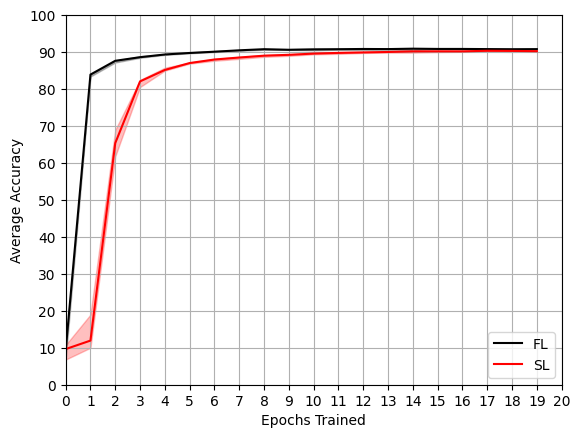
\includegraphics[width=300px]{aeg1}
	\caption{Comparing Accuracy of FL and SL with 6000 Data Samples per Node}
	\label{aeg1}
\end{figure}

\begin{figure}[H]
	\center{\textbf{Accuracy by Training Step for 1000 Samples}} \\
	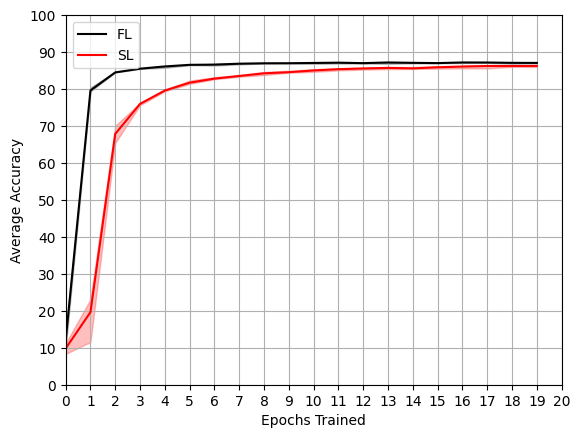
\includegraphics[width=300px]{aeg2}
	\caption{Comparing Accuracy of FL and SL with 1000 Data Samples per Node}
	\label{aeg2}
\end{figure}

\begin{figure}[H]
	\center{\textbf{Accuracy by Training Step for 100 Samples}} \\
	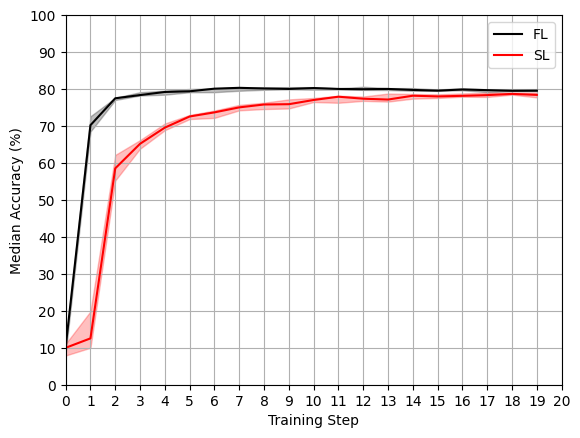
\includegraphics[width=300px]{aeg3}
	\caption{Comparing Accuracy of FL and SL with 100 Data Samples per Node}
	\label{aeg3}
\end{figure}

\todo{Describe the above graphs}

\section{Dense Network Performance with Node Dropout}

the same but this time dropout nodes. Try with and without filtering to show that it increases fault tolerance

To do this, test where a certain number of nodes drop out at step 1, 2, 3, etc

\section{Sparse Network Performance}

can only test SL here (i guess you could take average number of neighbours and do fl on that too)

\section{Sparse Network Performance with Dropout}